\section{DIP}
\label{sec:algorithms:dip}

\begin{figure}
	\centering
	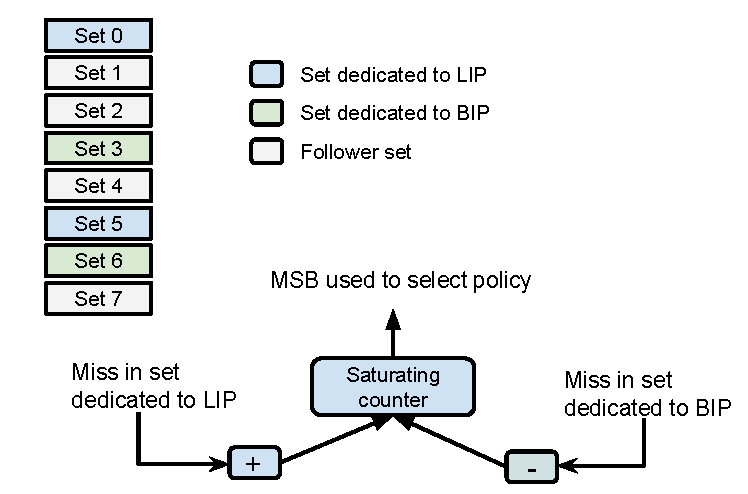
\includegraphics[width=\textwidth]{figures/algorithms/DIP_architecture}
	\caption{DIP set-dueling architecture}
	\label{fig:algorithms:dip:set_dueling}
\end{figure}

\begin{figure}
	\centering
	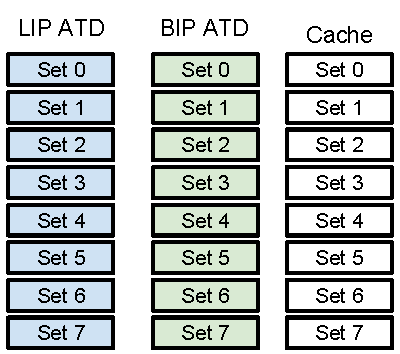
\includegraphics[width=\textwidth]{figures/algorithms/DIP_atd_architecture}
	\caption{DIP ATD architecture}
	\label{fig:algorithms:dip:atd}
\end{figure}

Dynamic Insertion Policy (DIP)~\cite{Qureshi2007} was originally proposed by M. K. Qureshi et al. in 2007.
The DIP algorithm views the cache set as a stack, as in LRU.
Replacement and promotion policies are equal to LRU, DIP evicts the block at the LRU position, and following a cache hit a block moves to the MRU position.
In contrast to LRU, DIP is a combination of two insertion policies, the standard LRU insertion policy (LIP) and Binominal Insertion Policy (BIP).
LIP inserts new blocks at the MRU position.
BIP inserts new blocks either at the LRU position or with a small probability, $p = \frac{1}{32}$, at the MRU position. 
The overall DIP algorithm switches between the two insertion policies by always using the one that is expected to cause fewer cache misses.

By mostly inserting at the LRU position the BIP insertion policy can theoretically handle trashing memory access patterns.
BIP inserts most of the new blocks in the LRU position, and the upper part of the LRU stack can contain blocks that have been re-referenced.
In a trashing access pattern, this results in part of the working set residing in the upper part of the stack while rest is inserted at the LRU position and evicted at the next miss.
By sometimes inserting at the MRU position BIP will give blocks not referenced by the next miss a chance to stay in the cache. 
This will also force stale cache blocks in the upper part of the stack to move towards the LRU position.

The authors of DIP present several methods to detect the best replacement algorithm, one of them is set-dueling.
Set-dueling is implemented by having some sets of the cache always use BIP and some always use LIP.
A counter tracks the performance of the dueling sets.
Misses in LRU sets will increment the counter and misses in BIP sets will decrement the counter.
The MSB of the counter can then be used to select the optimal algorithm.
If the MSB is one, an overweight of misses in LRU sets are occurring, and BIP is the optimal algorithm. 
If the MSB is zero, then an overweight of BIP misses are occurring, and LRU is the optimal algorithm.
Figure~\ref{fig:algorithms:dip:architecture} shows the set dueling and algorithm selection algoritecture suggested by M. K. Qureshi et al.
In the figure sets x, y and z are dueling sets for LIP while x, y, and z are dueling sets for BIP.
All other sets are follower sets, meaning that they utilize the algorithm indicated by the selection logic.

Another solution is to utilize two Auxilliary Tag Directories (ATDs) which is a structure equal to the Tag directory of the cache itself.
The two ATDs run one algorithm each, and all cache accesses are also executed on the ATDs.
Again a counter controlled by misses in either ATD is used to select the optimal algorithm for the main cache.
The main advantage of using a ATD is that all available information is used when selecting between BIP and LIP.
Also the entire cache will always use the best algorithm, where in set-dueling a faction of the sets will always run the non-optimal algorithm.
However, ATDs required additional storage space, where set-dueling uses the existing store space and only requires counters and algorithm selection logic.